% Autor: Leonhard Segger, Alexander Neuwirth
% Datum: 2017-10-30
\documentclass[
	% Papierformat
	a4paper,
	% Schriftgröße (beliebige Größen mit „fontsize=Xpt“)
	12pt,
	% Schreibt die Papiergröße korrekt ins Ausgabedokument
	pagesize,
	% Sprache für z.B. Babel
	ngerman
]{scrartcl}

% Achtung: Die Reihenfolge der Pakete kann (leider) wichtig sein!
% Insbesondere sollten (so wie hier) babel, fontenc und inputenc (in dieser
% Reihenfolge) als Erstes und hyperref und cleveref (Reihenfolge auch hier
% beachten) als Letztes geladen werden!

% Silbentrennung etc.; Sprache wird durch Option bei \documentclass festgelegt
\usepackage{babel}
% Verwendung der Zeichentabelle T1 (Sonderzeichen etc.)
\usepackage[T1]{fontenc}
% Legt die Zeichenkodierung der Eingabedatei fest, z.B. UTF-8
\usepackage[utf8]{inputenc}
% Schriftart
\usepackage{lmodern}
% Zusätzliche Sonderzeichen
\usepackage{textcomp}

% Mathepaket (intlimits: Grenzen über/unter Integralzeichen)
\usepackage[intlimits]{amsmath}
% Ermöglicht die Nutzung von \SI{Zahl}{Einheit} u.a.
\usepackage{siunitx}
% Zum flexiblen Einbinden von Grafiken (\includegraphics)
\usepackage{graphicx}
% Abbildungen im Fließtext
\usepackage{wrapfig}
% Abbildungen nebeneinander (subfigure, subtable)
\usepackage{subcaption}
% Funktionen für Anführungszeichen
\usepackage{csquotes}
\MakeOuterQuote{"}
% Zitieren, Bibliographie
\usepackage{biblatex}


% Zur Darstellung von Webadressen
\usepackage{url}
%chemische Formeln
\usepackage[version=4]{mhchem}
% siunitx: Deutsche Ausgabe, Messfehler getrennt mit ± ausgeben
\usepackage{floatrow}
\floatsetup[table]{capposition=top}
\usepackage{float}
% Verlinkt Textstellen im PDF-Dokument
\usepackage[unicode]{hyperref}
% "Schlaue" Referenzen (nach hyperref laden!)
\usepackage{cleveref}
\sisetup{
	locale=DE,
	separate-uncertainty
}
\bibliography{14Mo_O3_18-06-2018_References}

\begin{document}
	
	\begin{titlepage}
		\centering
		{\scshape\LARGE Versuchsbericht zu \par}
		\vspace{1cm}
		{\scshape\huge O3 - Polarisation \par}
		\vspace{2.5cm}
		{\LARGE Gruppe 14Mo \par}
		\vspace{0.5cm}
		
		{\large Alexander Neuwirth (E-Mail: a\_neuw01@wwu.de) \par}
		{\large Leonhard Segger (E-Mail: l\_segg03@uni-muenster.de) \par}
		\vfill
		
		durchgeführt am 18.06.2018\par
		betreut von\par
		{\large Kristina Mühlenstrodt}
		
		\vfill
		
		{\large \today\par}
	\end{titlepage}
	\tableofcontents
	\newpage


	\section{Kurzfassung}
	Es werden mehrere Experimente durchgeführt, die den Einfluss verschiedener optischer Elemente auf die Polarisationsrichtung eines Laserstrahls untersuchen.
	Zunächst wird die Abhängigkeit der Intensität vom Winkel zwischen Polarisator und Analysator untersucht.
	Erwartet wird hier, dass diese das Gesetz von Malus erfüllt.
	Dies kann jedoch nicht eindeutig bestätigt werden.
	Bei Untersuchung einer $\lambda /2$-Platte wird erwartet, dass zwischen Winkel der  $\lambda /2$-Platte und ursprünglicher Polarisationsrichtung und Winkel der resultierenden Polarisationsrichtung ein Faktor 2 liegt.
	Die Messung ergibt einen Wert von \SI{1,88\pm 0,006}{}.
	Die Untersuchung der Intensität von an einer Glasplatte reflektierten Strahlung in Abhängigkeit vom Einfallswinkel ergibt den charakteristischen Verlauf für parallel und senkrecht polarisiertes Licht.
	Aus dem Minimum der Intensität bei parallel polarisiertem Licht lässt sich der Brechungsindex des Glases bestimmen.
	Dies ergibt einen Wert von \SI{1,43 \pm 0,05}{}, was innerhalb der Unsicherheiten mit dem Literaturwert für Quarzglas übereinstimmt.
	Auch die Annahme, dass die Reflexion die Polarisationsrichtung nicht ändert, kann bestätigt werden.
	Die Untersuchung der Polarisationsrichtungsänderung durch Zuckerlösung verschiedener Konzentrationen bestätigt, dass Zuckerlösung eine linksdrehende Substanz ist.
	Außerdem kann innerhalb der Limitierungen des Versuchsaufbaus die Konzentration einer unbekannten Zuckerlösung bestimmt werden.
	Zuletzt wird ein Kalkspatkristall betrachtet.
	Die Messung der Polarisation der austretenden Strahlen lässt Rückschlüsse auf die Lage der optischen Achse des Kristalls zu.
	%ca. 203 Wörter
	\section{Methoden}
	Zunächst werden Laser, zwei Polarisationsfilter und Photodiode in dieser Reihenfolge in einer Linie auf der optischen Bank positioniert.
	Bei fester Polarisationsrichtung durch den ersten Filter wird der zweite Filter schrittweise gedreht und so die Intensität in Abhängigkeit vom Winkel zwischen den Durchlassrichtungen bestimmt.
	
	Jetzt wird eine $\lambda /2$-Platte zwischen die Filter gebracht.
	Es wird die $\lambda /2$-Platte gedreht und abhängig vom Winkel dieser relativ zum Polarisator die Polarisation des aus der $\lambda /2$-Platte austretenden Strahls bestimmt.
	Dazu wird durch Drehung des Polarisationsfilters vor der Diode das Maximum der Intensität gesucht.
	
	Dann wird eine Glasplatte in den Strahlengang gebracht und der Polarisationsfilter, der als Analysator fungiert, und die Photodiode wie in \cref{fig_reflexion_aufbau} auf einem beweglichen Arm positioniert.
	Die Arme werden jeweils so positioniert, dass sie in gleichem Winkel zur Glasplatte stehen.
	Der Einfallswinkel wird schrittweise erhöht die Intensität in Abhängigkeit vom Einfallswinkel gemessen.
	Dies wird einmal mit parallel und einmal mit senkrecht zur Tischebene polarisiertem Licht durchgeführt.
	Außerdem wird mit dem Analysator untersucht, ob der Laserstrahl nach der Reflexion seine Polarisationsrichtung behalten hat.
	
	\begin{figure}[H] 
		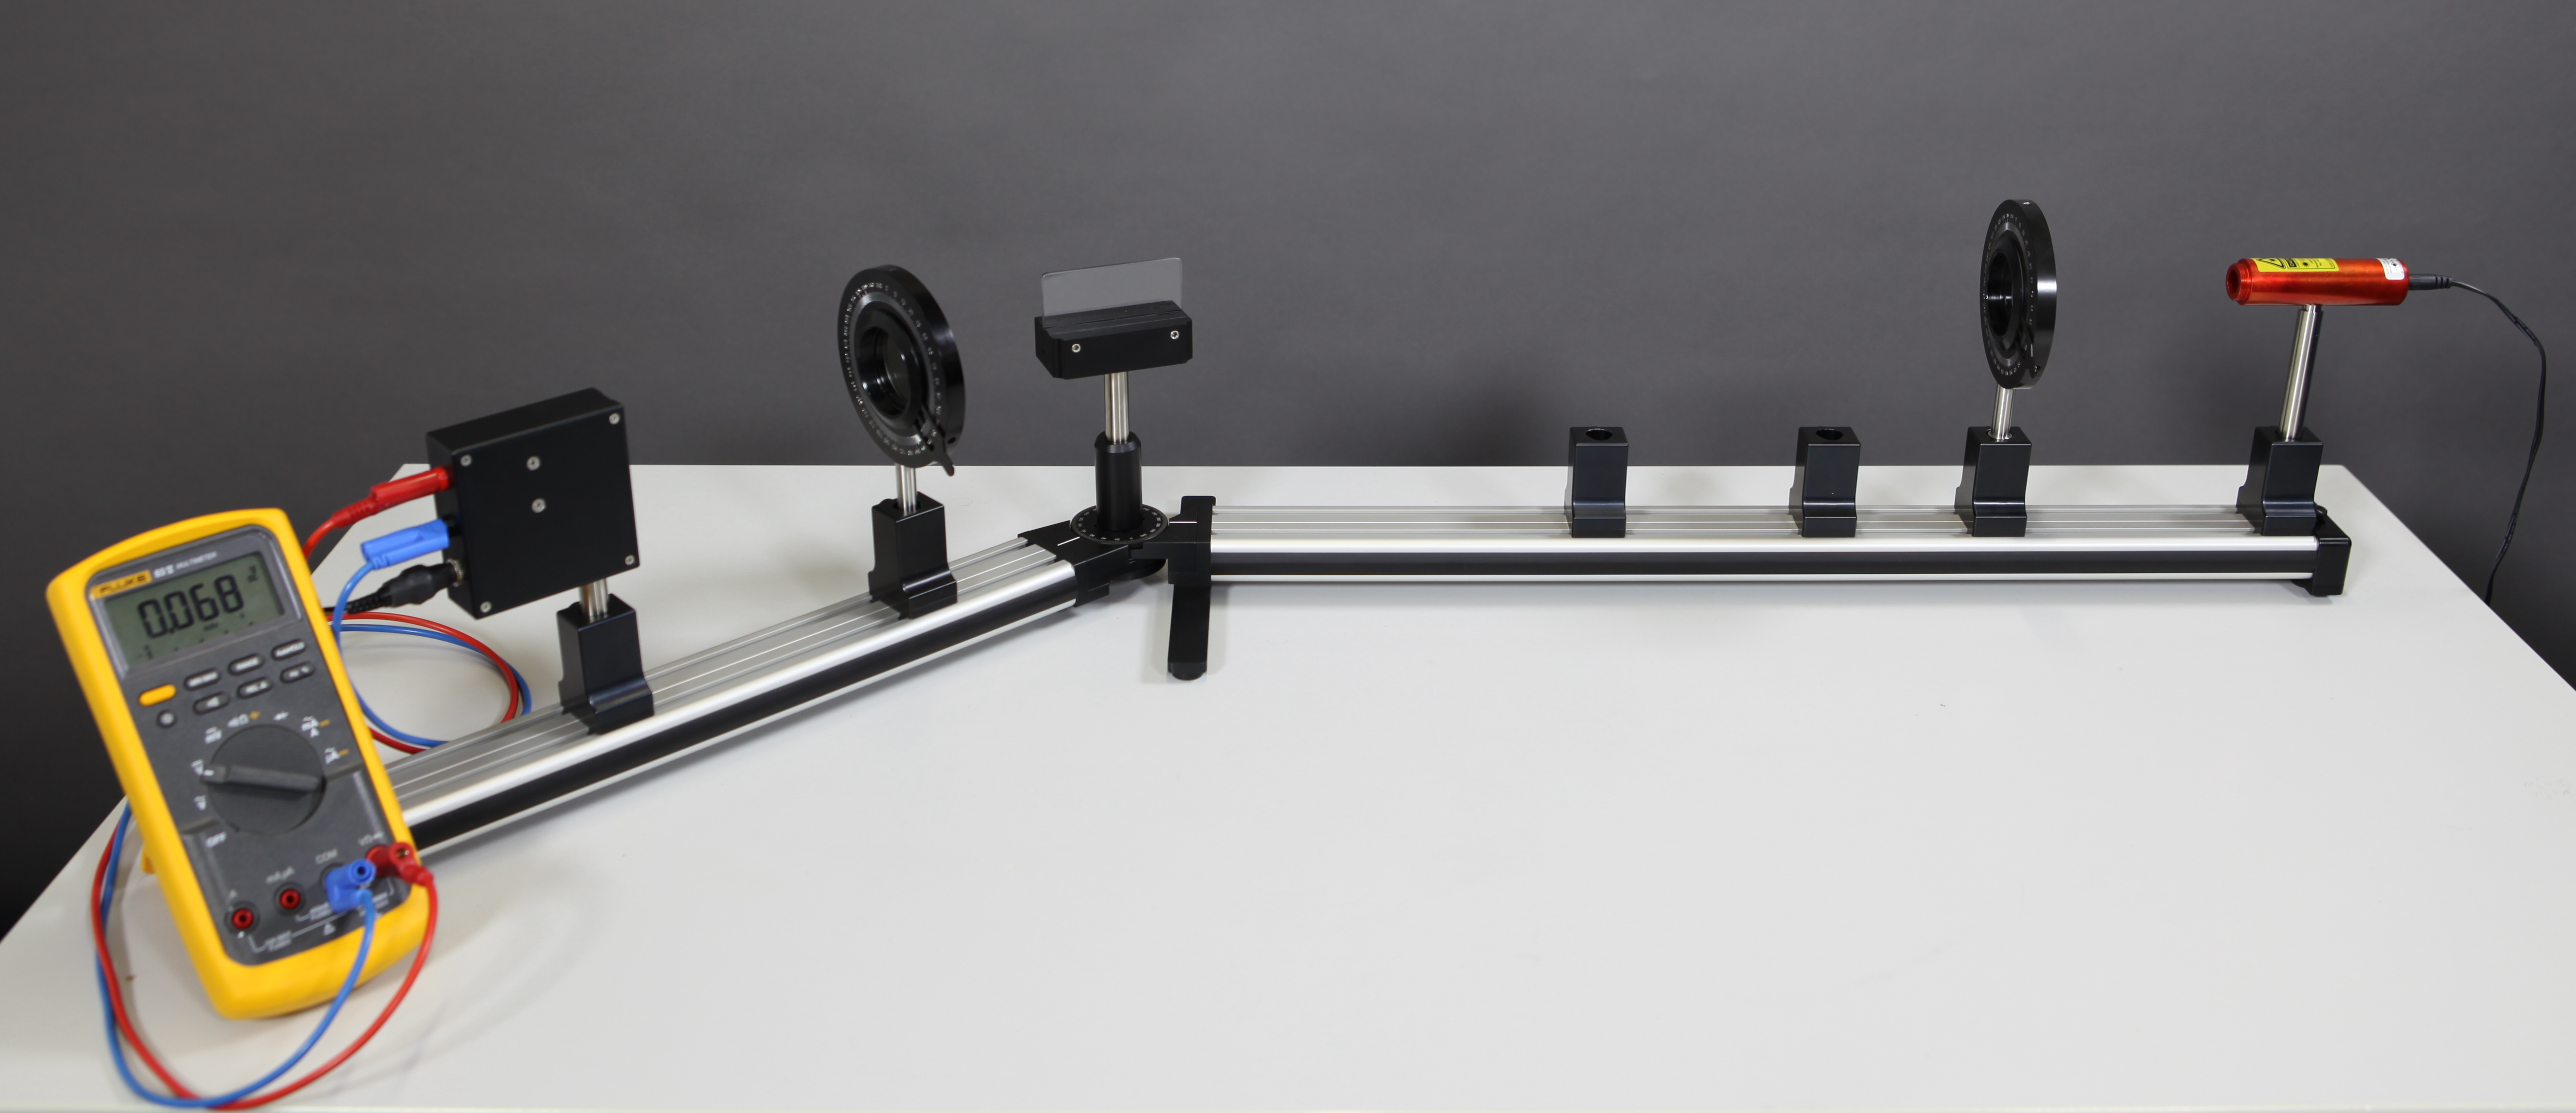
\includegraphics[width=1\textwidth]{fig_reflexion_aufbau}
		\centering
		\caption{Aufbau bei Messung des Reflexionsvermögens einer Glasplatte bei parallel und senkrecht polarisiertem Licht. \cite{aufbau_reflexion}} 
		\label{fig_reflexion_aufbau}
		\centering
	\end{figure}
	
	Nun werden die optischen Elemente wieder in eine Achse gebracht und die Glasscheibe durch eine Halterung für Glasröhren ersetzt.
	Es wird wie oben die Polarisationsrichtungsänderung durch Glasröhren mit sechs Zuckerlösungen verschiedener Konzentration untersucht.
	Dabei sind die Konzentrationen von fünf der Lösungen bekannt.
	Dies wird mehrfach durchgeführt.
	
	Zuletzt wird anstelle der Glasröhren ein Kalkspatkristall in den Strahlengang gebracht.
	Es wird für parallel und senkrecht polarisiertes Licht die Änderung der Polarisationsrichtung durch den Kalkspat gemessen.
	
	\section{Ergebnisse und Diskussion}
	%TODO Unsicherheiten
	
	%TODO Einflüsse von veränderten Parametern auf Messung
	\subsection{Unsicherheiten} %TODO GGF IN DATENANYLSY
	Die Unsicherheiten werden gemäß GUM ermittelt. 
	Außerdem wird für Unsicherheitsrechnungen die Python Bibliothek "uncertainties" verwendet.
	\begin{description}
		\item[Photodiode/Multimeter:] Der Messwert der Photodiode wird auf einem Multimeter abgelesen. 
			Das Multimeter zeigt die Spannung mit 3 Nachkommastellen an. 
			Es ergibt sich also eine Unsicherheit von \SI{0,0003}{V} (rechteckige WDF).
			Bei allen Messungen außer dem Überprüfen des Gesetz von Malus und der Untersuchung der $\lambda/2$-Platte müsste die Photodiode nach jedem Verändern der Systemparameter rejustiert werden, damit der Laserstrahl wieder mittig auf die Photodiode trifft. 
			Daher wird für diese Messungen die Unsicherheit mit \SI{0,003}{V} abgeschätzt. %TODO unsihcherheit ggf höher
		\item[Winkelmessung:]  Die Winkel werden mit dem Auge anhand einer Skala abgelesen, wobei die Unsicherheit für den Polarisator/Analysator und die $\lambda/2$-Platte \SI{0,4}{\degree} beträgt. 
			Beim Einstellen des Analysatorwinkels bei der Bestimmung der Konzentration der Zuckerlösung ändert sich die gemessene Intensität des transmitierten Strahls kaum in Abhängigkeit von dem Winkel nahe dem Maximum. 
			Insofern wird eine Unsicherheit von \SI{2}{\degree} angenommen.
			Die Skala des Winkelmessarmes ist kleiner als die der Polarisatoren und der Arm hat beim Konfigurieren etwas Spielraum. 
			Folglich wägen wir die Unsicherheit mit \SI{0,8}{\degree} ab.
	\end{description} 

	\subsection{Gesetz von Malus}
	\subsubsection{Beobachtung und Datenanalyse}
	Das Multimeter, das an die Photodiode angeschlossen ist, zeigt eine Spannung von \SI{0,060+-0,001}{V} an, während der Laser ausgeschaltet war.
	Beim Vergleichen der Intensitäten mit nur einem Polarisator zeigt sich, dass der Laser einen höheren p-polarisierten als s-polarisierten Anteil erzeugt.
	In \cref{fig_Malus1} ist die Lichtintensität gegen den Analysatorwinkel $\alpha$ relativ zum Polarisator aufgetragen.
	Der Analysatorwinkel wird in \SI{10}{\degree}-Schritten von \SI{-90}{\degree} bis \SI{90}{\degree} variiert.

	\begin{figure}[H]
		\includegraphics[width=0.7\textwidth]{fig_Malus1}
		\centering
		\caption{Ein Laserstrahl wird zuerst durch einen Polarisator und dann durch einen Analysator gelenkt. 
		Der Winkel zwischen Polarisator und Analysator ist auf der X-Achse dargestellt. 
		Hinter dem Analysator wird mit einer Photodiode und eine Multimeter die Intensität gemessen. 
		Diese ist in willkürlichen Einheiten dargestellt. 
		Die Unsicherheiten sind kleiner als die Symbolgröße.} 
		\label{fig_Malus1}
		\centering
	\end{figure}

	\subsubsection{Diskussion}
	
	Eigentlich ist in \cref{fig_Malus1} gemäß
	\begin{equation}
		I = I_0 \cos^2 \alpha
		\label{eq_malus}
	\end{equation}
	ein Verlauf der Intensität in Form eines quadrierten Kosinus zu erwarten.
	Dies lässt sich aufgrund der starken Abflachung an der Oberseite und der mangelnden Abflachung an den Rändern nicht bestätigen.
	Grund für die Abflachung zwischen \SI{-30}{\degree} und \SI{30}{\degree} und nicht exakte Symmetrie der Kurve kann sein, dass die Sättigung der Diode erreicht wurde und deshalb eine erhöhte Intensität nur zu einer geringfügig erhöhten Spannung führt.
	Die mangelnde Abflachung bei großen Analysatorwinkeln kann mit mangelnder Exaktheit der Filter zusammenhängen.
	Wenn diese bei einem Winkel von \SI{90}{\degree} zwischen Polarisator und Analysator noch große Teile der Strahlung passieren lassen, kann das dazu führen, dass der erwartete Abfall auf $I = 0$ nicht gemessen werden kann.
	Hierauf hat auch thermische Effekte in der Diode und die mangelnde Abdunklung des Raums einen Einfluss, da sich veränderndes Umgebungslicht einen störenden Einfluss haben kann. %TODO not sure mit den thermischen Effekten
	
	\subsection{$\lambda/2$-Platte}
	\subsubsection{Beobachtung und Datenanalyse}
	%Die e wird in \SI{45}{\degree}-Stellung zwischen Polarisator und Analysator positioniert.  
	%Der Winkel des Analysators wird so gewählt, dass die Photodiode einen maximale Intensität misst. %TODO das ist ultra doppelt
	Wenn eine Winkeldifferenz von \SI{45+-0,4}{\degree} zwischen Polarisator und $\lambda/2$-Platte eingestellt ist, wird ein Analysatorwinkel von \SI{89+-0,4}{\degree} gemessen.
	In \cref{fig_lambda} sind gegen einige andere Stellungen der $\lambda/2$-Platte die resultierenden Analysatorwinkel aufgetragen.

	\begin{figure}[H]
		\includegraphics[width=0.7\textwidth]{fig_lambda}
		\centering
		\caption{Ein Laser strahlt als erstes durch einen Polarisator. 
		Darauf folgt eine $\lambda/2$-Platte, die mit einem Winkel $\alpha$ relativ zur Polarisation des eintreffend Strahls ausgerichtet wurde. 
		Vor der Photodiode befindet sich ein Analysator, der so justiert wurde, dass die gemessene Intensität maximal wird.
		Der Winkel $\beta$ des Analysators relativ zum Polarisator wird gegen den Plattenwinkel $\alpha$ aufgetragen.
		Es wird ein linearer Fit durchgeführt.
		Die Unsicherheiten sind kleiner als die Symbolgröße.}
		\label{fig_lambda}
		\centering
	\end{figure}

	\subsubsection{Diskussion}
	In der Einführung wurde für einen Laserstrahl bei der Transmission durch eine $\lambda/2$-Platte eine Drehung der Polarisationsebene um $\Delta\beta=2\alpha$ vorhergesagt, wobei $\alpha$ der Drehwinkel der Platte relativ zur Polarisationsrichtung ist.
	Um dies überprüfen zu können, wurde ein linearer Fit durchgeführt.
	Die Steigung $a=\SI{1,88+-0,06}{}$ gibt den Faktor zwischen $\Delta\beta$ und $\alpha$ an.
	Hier liegt die Erwartung von 2 innerhalb der doppelten Unsicherheit des Messwerts, weshalb der erwartete Zusammenhang nicht widerlegt werden kann.
	Die Abweichung kann an Verunreinigungen der optischen Elemente liegen.
	Da nicht bekannt ist, auf welche Wellenlänge die vorliegende $\lambda /2$-Platte abgestimmt ist, kann die Abweichung auch darauf zurückzuführen sein, dass sie nicht auf die exakte Wellenlänge des verwendeten Lasers ausgelegt ist.
	
	\subsection{Reflexionsvermögen}
	\subsubsection{Beobachtung und Datenanalyse}
	Es wird ein p bzw. s polarisierter Laserstrahl auf eine Glasplatte mit einem Einfallswinkel $\alpha$ gerichtet und die Intensität des reflektierten Strahls bestimmt.
	Zunächst wird mittels des Analysators vor der Photodiode überprüft, ob sich die Polarisationsrichtung geändert hat. 
	Die Spannung am Multimeter ändert sich nahezu nicht wenn die Polarisationsrichtung gleich der des einfallenden Strahls ist. 
	Ebenso wird die gemessene Intensität minimal für eine Winkeldifferenz von $\SI{\pm90}{\degree}$.
	In \cref{fig_pol} ist die Lichtintensität des reflektierten Lichts gegen den Einfallswinkel $\alpha$ von \SI{30}{\degree} bis \SI{85}{\degree} in \SI{5}{\degree}-Schritten aufgetragen.
	Dabei tritt das Problem auf, dass zwischen jeder Messung die Photodiode so rejustiert werden muss, dass der Laserstrahl diese zentriert trifft.
	Es ist ein deutliches Minimum für die Reflexion von p-polarisiertem Licht erkennbar.
	Laut der Einführung wird im Brewsterwinkel $\alpha_B$ kein p-polarisiertes Licht reflektiert.
	Folglich beträgt der Brewsterwinkel ca. $\alpha_B = \SI{55+-1}{\degree}$.
	Außerdem ist \cref{eq_brech} zur Bestimmung des Brechungsindex gegeben.
	\begin{equation}
		n= \tan(\alpha_B)
		\label{eq_brech}
	\end{equation}
	\begin{equation}
		u(n) = \frac{1}{\cos(\alpha_B)^2} \cdot u(\alpha_B)
		\label{eq_unsicher}
	\end{equation}
	Es ergibt sich ein Brechungsindex $n = \SI{1,43 +- 0,05}{}$

	\begin{figure}[H]
		\centering
		\begin{subfigure}[t]{0.5\textwidth}
			\centering
			\includegraphics[width=1\textwidth]{fig_ppol}
			\label{fig_ppol}
			\caption{p-polarisiertes Licht}
		\end{subfigure}%
		\begin{subfigure}[t]{0.5\textwidth}
			\centering
			\includegraphics[width=1\textwidth]{fig_spol}
			\label{fig_spol}
			\caption{s-polarisiertes Licht}
		\end{subfigure}
		\caption{
			\label{fig_pol}%
		Ein Laserstrahl wird nach einem Polarisator an einem Glas unter dem Winkel $\alpha$ reflektiert und die Intensität des reflektierten Lichts wird gemessen. 
		Es wird p- und s-polarisiertes Licht untersucht.
		Die Unsicherheiten sind kleiner als die Symbole.}
		\centering

	\end{figure}

	\subsubsection{Diskussion}
	Dass sich die Polarisationsrichtung durch die Reflexion nicht ändert, kann bestätigt werden, da bei stichprobenartiger Messung das Maximum der Intensität bei Drehung des Analysators beim am Polarisator eingestellten Winkel liegt.
	Außerdem entsprechen die Verläufe der Intensität in Abhängigkeit von Einfallswinkel und Polarisationsrichtung in \cref{fig_pol} den gemäß der Einführung erwarteten Verläufen.
	Das Minimum der Reflexion von p-polarisiertem Licht am Brewsterwinkel ist eindeutig zu erkennen.
	Der daraus bestimmte Brechungsindex von \SI{1,43 \pm 0,05}{} stimmt innerhalb der Unsicherheiten mit dem Literaturwert von \SI{1,46}{} bei einer Wellenlänge von \SI{589,3}{nm} überein. \cite{quarz_brech}
	Verwendet wurde ein Laser mit einer Wellenlänge von ca. \SI{650}{\nano \meter}.
	Der Brechungsindex ändert sich im Allgemeinen nicht hinreichend stark mit der Wellenlänge, als dass dieser Literaturwert hier nicht anwendbar wäre.

	\subsection{Zuckerkonzentration}
	\subsubsection{Beobachtung und Datenanalyse}
	Bei Untersuchung der Zuckerlösungen sind von den sechs Lösungen sind fünf Konzentrationen bekannt.
	Unter der Annahme, dass sich die Polarisation in der Flüssigkeit um nicht mehr als $\pi$ dreht, ließ sich feststellen, dass alle Flüssigkeiten die Polarisation links gedreht haben und somit auch dass die Zuckerlösung linksdrehend sind.
	In der Einführung wurde ein proportionaler Zusammenhang zwischen dem Drehwinkel $\alpha$ und der Flüssigkeitslänge $l$ und der Konzentration $c$ nahegelegt.
	\begin{equation}
		\alpha \propto c \cdot l
	\end{equation}
	Folglich wurde in \cref{fig_zucker} ein linearer Fit für die bekannten Konzentrationen berechnet.
	In der Graphik sind außerdem horizontale Geraden, die den Drehwinkel der unbekannten Flüssigkeit beschreiben.
	Der Mittelwert der vier Messungen der unbekannten Flüssigkeit ist $\alpha=\SI{26,75+-1,11}{\degree}$.
	Die Funktionsgleichung $ax+b=\alpha$ lässt sich nach x, also der Konzentration, umformen:
	\begin{equation}
		c = \frac{\alpha-b}{a}
	\end{equation}
	\begin{equation}
		u(c) = \sqrt{ \left(\frac{u(\alpha)}{a}\right)^2 + \left(\frac{u(b)}{a}\right)^2 + \left(\frac{c \cdot u(a)}{a}\right)^2}
	\end{equation}
	Die somit bestimmte Zuckerkonzentration $c$ beträgt $\SI{21,8+-1,9}{g/cm^3}$.


	\begin{figure}[H]
		\includegraphics[width=0.7\textwidth]{fig_Zucker}
		\centering
		\caption{Ein polarisierter Laser strahlt durch Glasröhren der gleichen Länge, welche mit verschieden konzentrierten Zuckerlösungen gefüllt sind. 
		Am Analysator vor der Photodiode lässt sich durch Variation des relativen Winkels zum Polarisator der Drehwinkel bestimmen, der durch die Flüssigkeit zustande kommt.
		Die Röhren werden von beiden Seiten untersucht (zwei Messpunkte pro Konzentration), sodass die Fehler durch die Glasröhren minimiert werden.
		Die horizontalen Geraden sind die Messungen der unbekannten Konzentration und aus dem Schnittpunkt mit dem linearen Fit ergibt sich die Konzentration.
		Die Unsicherheit der unbekannten Konzentration ist nicht dargestellt. Sie beträgt ebenfalls \SI{2}{\degree}.
		}
		\label{fig_zucker}
		\centering
	\end{figure}

	\subsubsection{Diskussion}
	Zunächst lässt sich feststellen, dass, wie nach der Einführung erwartet, Zuckerlösung eine linksdrehende Substanz ist.
	Da für die unbekannte Zuckerlösung kein Referenzwert bekannt ist, kann nicht überprüft werden, ob der gemessene Wert mit diesem übereinstimmt.
	Dennoch kann die Präzision dieser Art von Messung angezweifelt werden, da, wie in \cref{fig_zucker} zu erkennen ist, eine Wiederholung der Messung mit derselben Zuckerlösung einen signifikant abweichenden Messwert ergibt.
	
	\subsection{Kalkspatkristall}
	\subsubsection{Beobachtung und Datenanalyse}
	Auf einen Kalkspatkristall wird linear polarisiertes Licht gestrahlt.
	In dem Kristall sind mehrere Reflexionseffekte sichtbar. 
	Am Analysator sind jedoch lediglich zwei Strahlen deutlich räumlich getrennt nahe der Verlängerung des einfallenden Lasers sichtbar.
	Die Photodiode wird auf jeweils einen der Strahlen ausgerichtet und mit dem Analysator lässt sich die Polarisation relativ zum einfallenden Strahl bestimmen.
	Bei p-polarisiertem Licht ergibt sich für den einen Strahl eine relative Verschiebung der Polarisation um \SI{-30+-1}{\degree} und für den anderen eine von \SI{48+-1}{\degree}.
	Es wird erneut gemessen nachdem der Kristall entlang des Lots zur Erdoberfläche um \SI{180}{\degree} gedreht wurde.
	Diese Messung ergibt Polarisationsänderungen um \SI{30+-1}{\degree} und \SI{-50+-1}{\degree}.
	Bei s-polarisiertes Licht zeigen sich Polarisationsänderung von \SI{53+-1}{\degree} und \SI{-33+-1}{\degree}.

	\subsubsection{Diskussion}
	Gemäß der Einführung ist ein Polarisationsunterschied von \SI{90}{\degree} zwischen dem ordentlichen und dem außerordentlichen Strahl zu erwarten.
	Dieser konnte nicht innerhalb der Unsicherheiten, aber immerhin innerhalb von ca. \SI{10}{\degree} festgestellt werden.
	Dass das Drehen des Kristalls um die Hochachse zu einer Verschiebung der Polarisationsrichtung der beiden Strahlen in die jeweils andere Richtung führt, spricht dafür, dass die optische Achse des Kristalls gedreht wurde.
	Dies kann also als Hinweis verstanden werden, dass die optische Achse des Kristalls in seiner Halterung in einem Winkel von \SI{30+-1}{\degree} oder \SI{49+-1}{\degree} von der Erdoberfläche weg zeigt.
	
	
	\section{Schlussfolgerung} %TODO mehr?
	%ich nehme an, hier darf man imperfekt
	Es konnten verschiedene Feststellung bezüglich der Wechselwirkung der untersuchten optischen Elemente und unterschiedlich polarisiertem Licht gemacht werden.
	Das Gesetz von Malus konnte nicht bestätigt werden.
	Um den Grund dafür zu finden müsste das Experiment mit einem gedämpften Laser wiederholt werden und bei großen Winkeln in geringeren Abständen die Intensität gemessen werden.
	Die Untersuchung einer $\lambda/2$-Platte erlaubte eine Bestätigung der Vorhersagen der Einführung für den Zusammenhang zwischen Winkel zwischen $\lambda/2$-Platte und Polarisator und Polarisation des austretenden Lichts.
	Die Messung der Intensität von an einer Glasscheibe reflektiertem, unterschiedlich polarisiertem Licht erlaubte die Bestimmung des Brewsterwinkels und dieser die Bestimmung des Brechungsindex der vorliegenden Glasplatte.
	Bei der Untersuchung des Kalkspatkristalls konnten nur Hinweise auf die Lage der optischen Achse gefunden werden.
	Für eine zielführendere Untersuchung wäre eine Einstellung zwischen paralleler und senkrechter Polarisation sinnvoll gewesen.
	Dann hätte sich vermutlich eine Einstellung finden lassen, bei der nur ein Strahl transmittiert wird, was den Rückschluss auf die Lage der optischen Achse möglich gemacht hätte.
	
	\printbibliography
\end{document}
